%!TEX root = project.tex

\chapter*{About this project}

\paragraph{Abstract}
This project is a stock price forecaster. It is a web application designed using Streamlit which is an open-source python framework specifically for creating web apps using data science, machine learning etc. The web app allows the user to select a stock from a list and select the number of years the price should be forecast. The current state of the stock is displayed in a table and the recent history is displayed in a graph. The app will then use machine learning to predict the closing price of the chosen stock in n number of years chosen by the user. The predicted data will then be presented in a manner similar to the current data with a table and graph indication the predicted price with a legend for the users ease of reading.
My GitHub can be found at: https://github.com/DeanMcG/4thYearProject

\paragraph{Authors}
There is a single author for this project, myself, Dean McGowan.

\chapter{Introduction}

\paragraph{The stock market is a platform where people can buy and sell shares of companies to gain ownership in a company, diversify assets, or make a profit. Currently 55\%\ of American's invest in the stock market \cite{statista}. In recent years the ease of access has improved significantly with the release or trading brokerage apps such as Robinhood developed by Baiju Bhatt. Traders can purchase stocks of companies they believe will be successful and grow. If they are correct the profits are only limited by how much they initially invest. Of course the same goes for losses also. The pandemic saw a tremendous fall and subsequent mighty rise in the stock market that shook traders globally. It was this series of unexpected market crash and rise that made me interested in the question 'Is it possible to predict the market's behaviour?'.}

\paragraph{Artificial intelligence is simply the discipline of attempting to bring human intelligence to machines through of use of pre-defined algorithms. }

\paragraph{Machine learning is one of the fastest growing sectors in the technology word right now. Between 2016 and 2022 the overall machine learning market has grown from \$\ 1 billion in 2016 to \$\ 8.81 billion in 2022 \cite{venturebeat}.
Machine learning is a field of artificial intelligence that focuses on using data and algorithms to mimic the way humans use their brains. This allows the machine to learn without specifically programming the rules it must follow. The models become more accurate over time as they 'learn' gradually. Machine learning typically requires vast amounts of data and pre-processing. There are a few different types of machine learning like supervised learning in which all data given to the model is labelled, unsupervised learning where none of the inputs are labelled and the model must decide upon its own classifications or rules and reinforcement learning where the model is 'rewarded' when correct as to steer it in the right direction.}

\paragraph{This project utilises a type of neural network called a 'recurrent neural network' or an 'RNN'. This relates to the way human intelligence learns and understands. Humans do not look at a sentence and take in each word as an individual item, they take in each word remembering the word before it to put it into context. The network has a persistence to it. }

\begin{center}    
    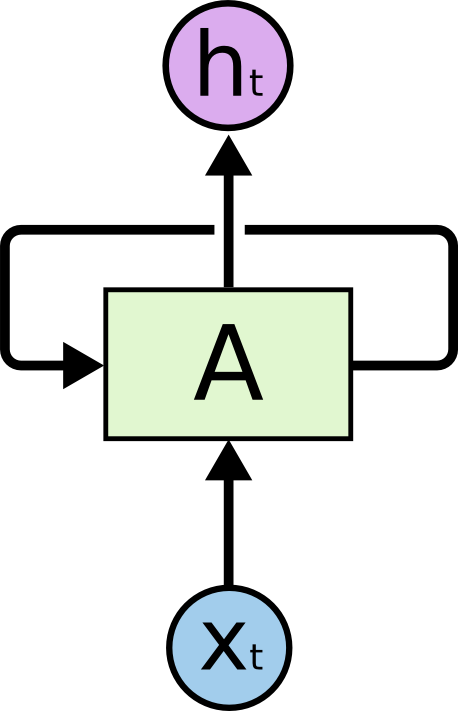
\includegraphics[scale=0.5]{img/RNN_diagram.png}
\end{center}

\paragraph{The figure above shows a neural network, labelled 'A'. Label 'Xt' is the input and label 'ht' is the output. As you can see the input is processed by the neural network and then an output is given, while simultaneously the output information is fed back into the neural network.}

\begin{center}    
    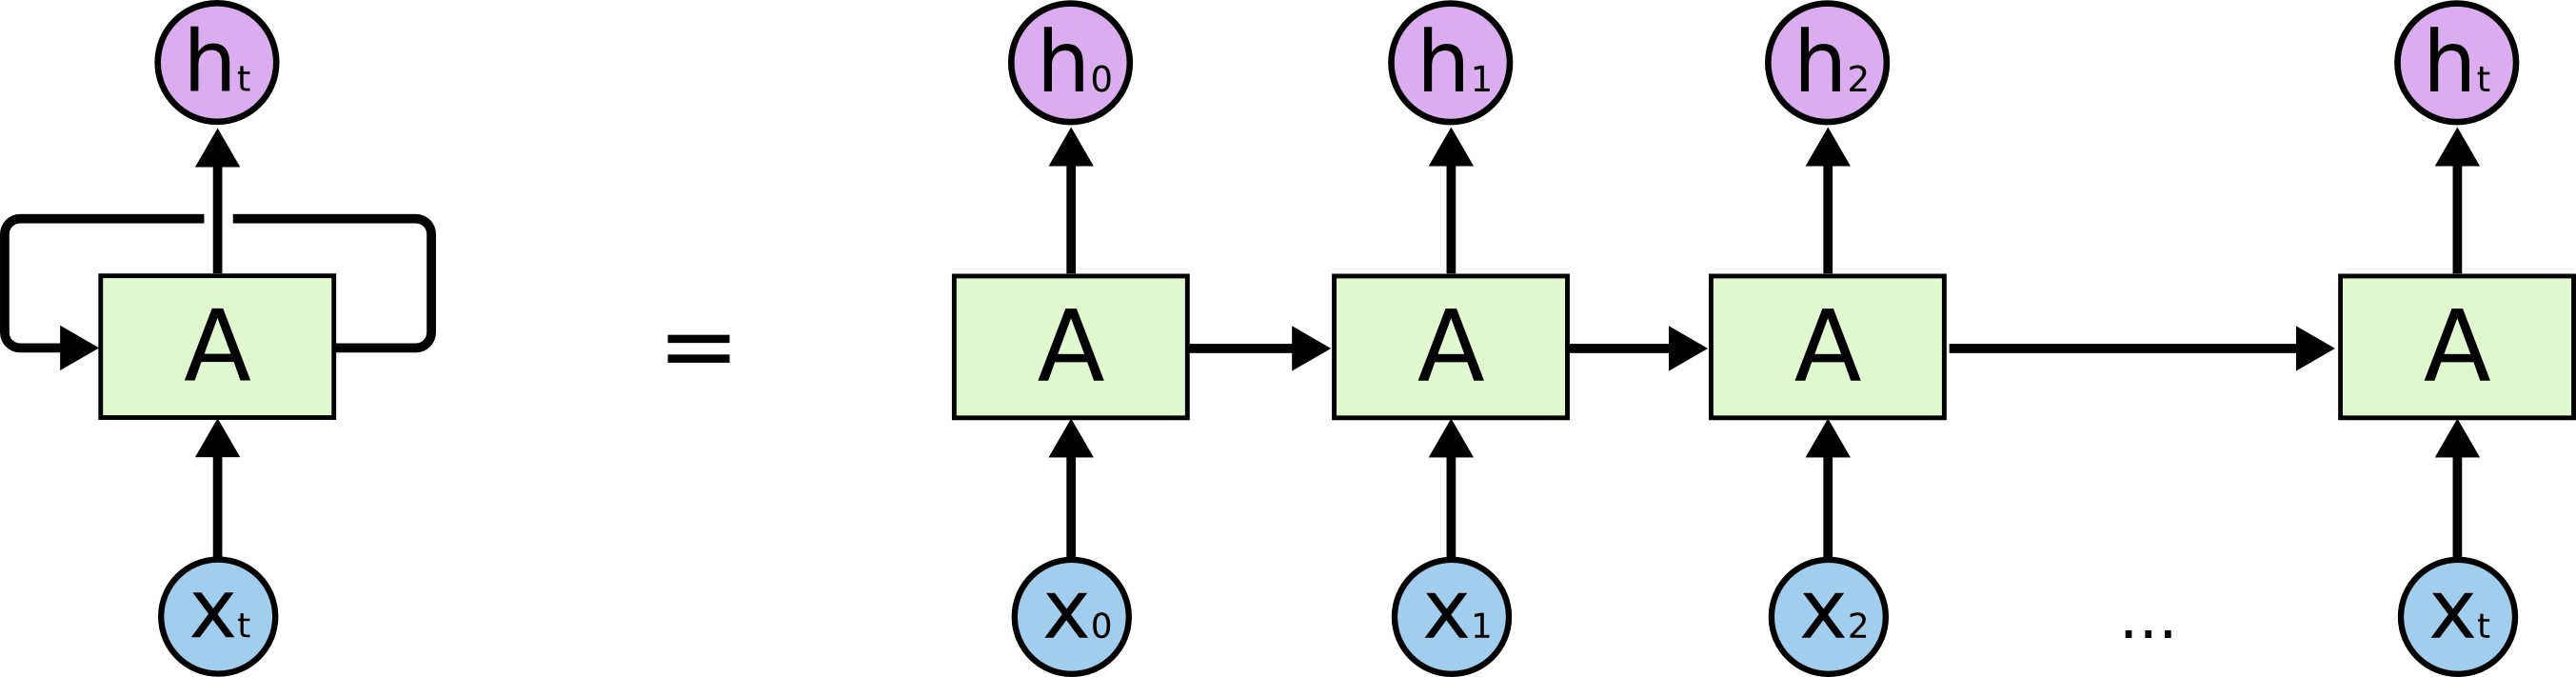
\includegraphics[scale=0.4]{img/RNN_expanded.png}
\end{center}

\paragraph{The figure above shows an RNN expanded out to visualise what is happening. It depicts that each neural network is passing on data to it's successor. You may note the visual similarity to a linked list. This is why RNNs are commonly used with sequential data. An RNN was the most effective choice for my work as the stock data I am working with is sequential.}

\paragraph{However, I did not use a standard RNN for my work. I used a very specific type of RNN called a 'Long Short Term Memory' network. To understand why I used this, I will describe the shortcomings of an RNN. An RNN is very efficient in using recent past data to learn and help process the current data. But a problem arises when they have to use data rather far back in the queue to process the current data. As an example, finishing the sentence "I went to the zoo and I saw a lot of...". An RNN will struggle to pull context from multiple words back to complete the sentence. Obviously the answer is 'animals' or a specific species. But this is only obvious to us and not the RNN. For my work I needed the network to recall more than just the past few days of stock data as they may not represent the true current performance, the stock may just have dipped for example, something frequent and completely normal for a stock to do.}

\paragraph{A 'Long Short Term Memory' network or an 'LSTM' is designed specifically to fix the long-term dependency problem present in a standard RNN. The LSTM design was first introduced in 1997 by two computer scientists Hochreiter and Schmidhuber. This type of network was created to remember data for long periods of time as it's natural behaviour.}


\begin{center}    
    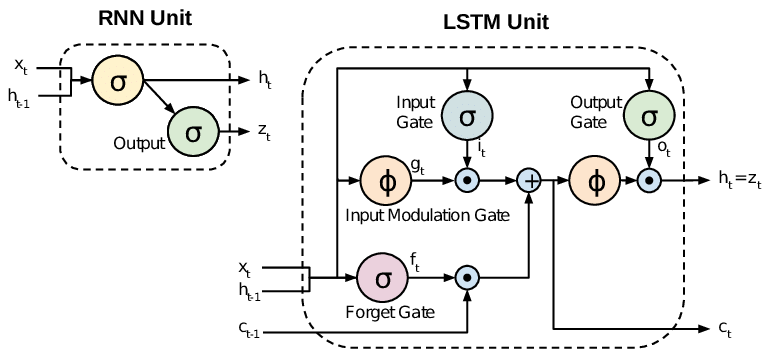
\includegraphics[scale=0.5]{img/RNN-Versus-LSTM.png}
\end{center}

\paragraph{All RNNs have the same topology. A chain of repeating neural networks as shown in figure 2. Each of these neural networks are quite simple as they will typically have a single tanh layer. A tanh layer is an activation function used to get the output of a node. In the case of a tanh function it will map the output somewhere between -1 and 1. }

\begin{center}
    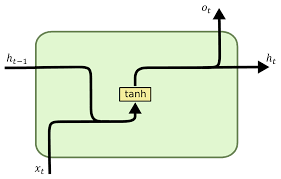
\includegraphics[scale=0.75]{img/RNN_single.png}
\end{center}

\paragraph{LSTMs have a similar topology to RNNs in that they share the chain-like structure, however, each module of the chain in an LSTM network is more complex than an RNN with each module containing four layers working together.}

\begin{center}
    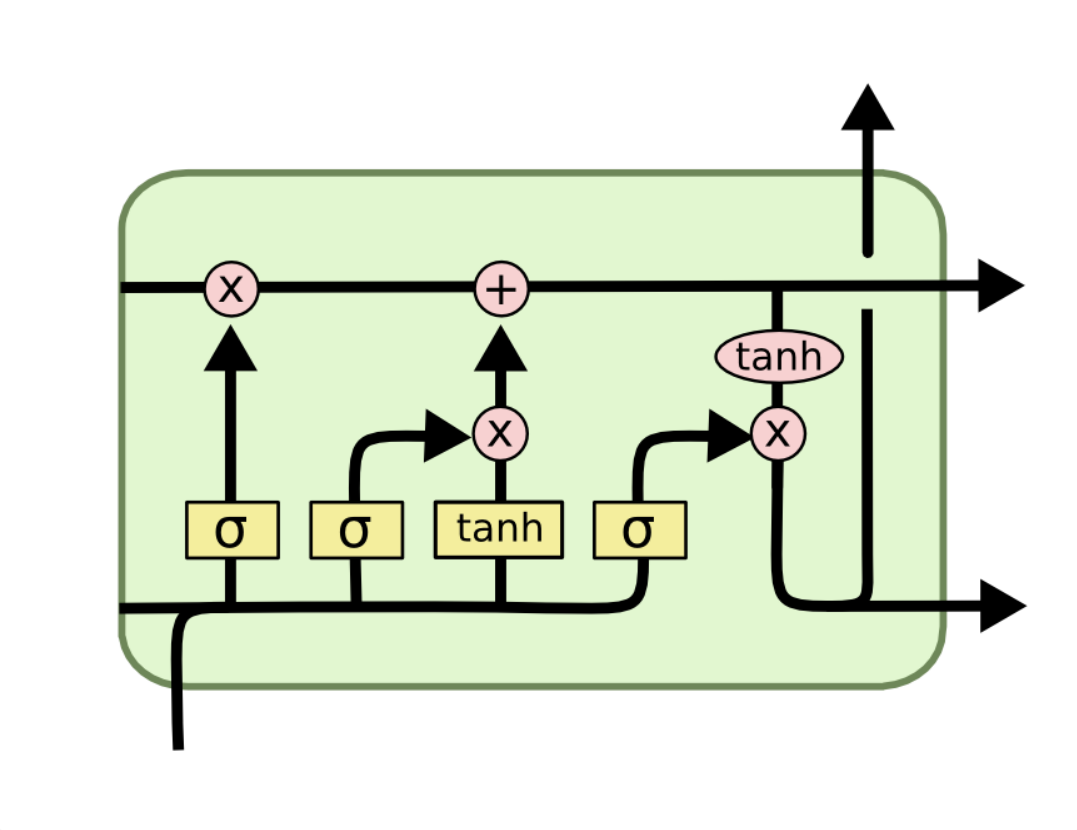
\includegraphics[scale=0.4]{img/LSTM_single.png}
\end{center}

\paragraph{In the above figure, the yellow boxes are neural network layers, the red circles are pointwise operations, and each line carries a vector. Where the lines split into two is copying and where they come together in concatenation.}

\paragraph{With the aforementioned in mind. My project is a web application based on the stock market that uses these machine learning techniques to take in stock information and predict the future price. In this development I wanted to cover these objectives: }

\begin{itemize}
    \item Develop a robust web application to a high standard using a technology that I have not yet developed with.
    \item Have my application read from and write to a database.
    \item Make my front-end user friendly and aesthetically pleasing for a good user experience.
    \item Allow users of the application to create accounts and log in to these accounts within the application
    \item Expand my knowledge of artificial intelligence, and more specifically machine learning techniques and applications.
    \item Develop an application in a manner similar to the industry standard like the agile methodology.
\end{itemize}

\chapter{Context}
\paragraph{The context of my application is to offer an easy to use UI that allows user to create an account, log-in, and use my web app. The web app offers stock data on popular stocks that the users can look at and generate a forecast of the stock data using a neural network.}

\subsection{Objectives}
\paragraph{The key objectives of this project are as follows:}

\begin{enumerate}
    \item \textbf{Sidebar:} The objective of the sidebar is to present the user with an easy to use and intuitive menu that allows them to navigate through three different pages (Home, Sign Up, and Login). The sidebar should be clearly labeled and the user should be able to understand the functionality regardless of their familiarity with application.
    
    \item \textbf{Home Page:} The home page should be the initial landing page of the application. Before the user is logged in they will be greeted with the home page that will direct the user on how to create an account or log in to a pre-existing account to access the main dashboard of the application.
    
    \item \textbf{Sign Up Page:} Once the user navigates to the sign up page, the objective for this is to get the user set up with an account consisting of a username and password. The page should also contain a submit button to create the account.
    
    \item \textbf{Login Page:} The objective of the login page is to get the user to sign in to their account using the previously created details. This page should have to be filled out and the information submitted before the user is allowed to access the main dashboard.
    
    \item \textbf{Dashboard:} The objective of the dashboard is to be a account only page in which users can select stocks from a list and have the data of these stocks displayed in a table and graphed. The user may also choose to generate a forecast of the stock data if they wish.
\end{enumerate}

\subsection{Following Chapters}

\paragraph{Methodology: Describes the methods in which I went about my project. The development approach, testing, why I chose the technologies used.}

\paragraph{Technology Review: I will give a review of each technology I used to create the application. I will discuss the technologies at a conceptual level, their standards, database models etc.}

\paragraph{System Design: I will cover the components of the application and how they work together.}

\paragraph{System Evaluation: }

\paragraph{My GitHub can be found at: https://github.com/DeanMcG/4thYearProject}


\chapter{Methodology}

\section{Development Method}
\paragraph{The development of this web application was completed using an agile approach. A list of requirements for the application was made in order of what needed to be done first .The development of these requirements  was split into approximately two week sprints. Often there would be gaps in the finishing of one sprint and the beginning of another as college work may have been more or less time consuming than average. Each sprint would have a list of deliverables and these deliverables would then be assessed at the end of the sprint. Refactoring and fixing bugs in the codebase took place after each sprint and this would be completed before the next sprint began.}

\paragraph{I chose this style of development as it kept me consistently adding to the codebase each week. Also meetings with my supervisor helped me stay on track with the development timeline. If I began to slip behind schedule the meetings were a good time to voice this and re-align where I was putting my time in. }

\section{Sprints}
\subsection{Sprint 1}
\paragraph{Sprint 1 consisted of researching possible ideas and fields in which to do my project. I looked at different technologies, applications of these technologies and what I would need to learn to complete the ideas I was considering.}

\subsection{Sprint 2}
\paragraph{Sprint 2 consisted of me finalising the idea for my project. I then drafted a proposal to show my supervisor and sent this to him. Once accepted I began to research artificial intelligence and what I needed to know to complete the tasks in my way. I took a 16 hour machine learning course on udemy.com given by a machine learning engineer in which I learned many theoretical and practical topics of machine learning. I found this gave me a good insight into what I needed for the development of my application.\cite{udemyml}}

\subsection{Sprint 3}
\paragraph{I used sprint 3 to test code in Jupyter notebook. I was fairly unfamiliar with Python so I used this time to play around with it and understand some of the standards, syntax, and functions. I also began researching what technology I would use to build the front-end. I finally decided on Streamlit after researching and building multiple prototypes with other options such as Flask.}

\subsection{Sprint 4}
\paragraph{I built the basic front-end in Streamlit in sprint 4 and like Python in sprint 3 I just played around with it, building things and then altering them. I done this to get familiar with the completely new technology to me at the time. I also created approximate work plans and timelines on functionality I wanted to implement and when I wanted these implemented by.}

\subsection{Sprint 5}
\paragraph{Sprint 5 was the creation of my Mongo database and populating it with relevant stock data. I also had to obtain the stock data from a reliable and trusted source. I used yahoo finance. Once the database was set up I then connected it to my application.}

\subsection{Sprint 6}
\paragraph{I worked on creating the first iteration of my LSTM model in sprint 6. This was the most difficult part that had done as of this time. I came across many errors both syntactical and logical during the development of this but I finally got it to work, however not accurately.}

\subsection{Sprint 7}
\paragraph{In sprint 7 I finalised the machine learning model and began trying to display it in a graph using MatPlotLib. This came with a few bugs that I had to dedicate a lot of time to fixing. But I found the problem and was able to visualise the data correctly now.}

\subsection{Sprint 8}
\paragraph{Not much work was done in sprint 8. I simply refactored code so it was tidier and was structured properly in functions.}

\subsection{Sprint 9}
\paragraph{Sprint 9 saw the finalisation of the front-end in Streamlit and the fixing of any previous bugs I had. I also began looking into how I could possibly add user authentication to the application.}

\subsection{Sprint 10}
\paragraph{Sprint 10 was the final sprint in which I developed the user authentication functionality and implemented it into the codebase. I also read up on Python virtual environments and refactored my coding environment to run in a virtual environment, I had to reinstall all the external libraries and packages but this made my application much more robust and less likely to break in the future.}

\section{Testing}
\subsection{PyTest}
\paragraph{PyTest is a python testing framework. It allows developers to write scalable and simple tests for APIs, UI, and databases. You can write many different types of test case from unit testing to full functional testing. I used PyTest to write unit tests for my code so I could be sure it was functional and doing what I needed it to before deploying it to the web app. Had I not done this and bugs had arisen, it would have been very time consuming going through a large codebase to pinpoint the root of the problem.}

\subsection{Black Box}
\paragraph{A lot of the testing on my application was done on the machine learning model used to predict the stock data. This testing was completely black box testing. Black box testing is testing software without knowing the functionality of the software. There was no way for me to know what the neural network was learning from the data I fed it and what points of data it used in it's predictions. All I could do for this was tweak my code and test until I was happy with the accuracy of the model.}

\subsection{Jupyter Notebook}
\paragraph{Jupyter notebook was also a large part of my testing methodology. It was very simple and quick to boot up a Jupyter notebook and test my code in there rather than trying to implement it into the application to see if it functioned correctly.}

\section{Version Control}
\paragraph{I used GitHub as the tool for my version control. I created a repository on GitHub and committed all design changes and development to said repository incrementally as I worked on the application over many months. GitHub allowed me to add messages to these commits which made it very easy to go back and look at specific additions to the codebase based on what I needed. GitHub offers the ability to rollback the project if necessary. I did not have to use this but it is a helpful feature nonetheless.}





\chapter{Technology Review}

\paragraph{In this section I will cover the technologies used to create my application. I will explain the technologies used, what purpose they served in my application, and my opinions of the technologies.}
\section{Data}
\paragraph{The following explains the technologies I utilised to read and write data to and from. SQLite when dealing with user details and MongoDB for stock data.}

\subsection{SQLite}
\paragraph{SQLite is a C library that I used to store the user data for my application. Through the use of SQL queries I could write to and read from an SQL database. SQLite is a robust database option, it is atomic, consistent, isolated, and durable even after crashes and power failures.\cite{sqlite} SQLite has the advantage of being file-based as opposed to SQL server and MySQL both of which are server-based databases. SQLite is often used in mobile applications because the technology is light and its support to relational database management. SQLite is also self contained so it does not require any external dependencies. SQLite has a wide range of supported platforms such as Android, iOS ,Mac, Linux, Solaris, and Windows.\cite{bhosale2015sqlite} }

\subsection{MongoDB}
\paragraph{MongoDB was used for the storing of stock data sourced from yahoo finance. MongoDB is a document oriented NoSQL database. MongoDB doe not use the traditional model of tables with rows and columns. Instead it utilises 'collections' which contain documents. These documents are made up of key-value pairs. MongoDB was very user friendly when setting up the collections and connecting to my application. My application reads data with every use as the user must choose a stock and view its current data at that time. These operations are handled quickly and with little no errors as far as I have experienced. MongoDB stores data in JSON(JavaScript Object Notation) format. JSON is very readable to someone viewing the data and is a highly supported format for representing data. For my application MongoDB stores many details of the stock such as: date, open price, high price, low price, close price, adjusted close price, and volume. It stores all of these for each stock on each day for approximately 1200 days and reads this information instantaneously. Pyhton's pymongo distribution made it very easy and fast to make a connection between my application and my Mongo database.}

\section{Logic}

\subsection{Python}
\paragraph{Python is a general purpose programming language. It is designed to be easily readable and removes a lot of the boilerplate code that comes with other languages. There are many reasons I chose to use this language for my project. Python is the go to language for AI development. Python offers a large number of libraries and frameworks that make the development much easier for the developer thus saving me a large amount of time. Time management was crucial with this project as I was the sole contributor to it. Python is very readable. The simplicity of the language allows a developer to quickly read through the codebase and get a grasp of what is happening. A lot of the code pertaining to the creation of my neural network is very difficult to understand conceptually but thanks to Python the code itself is very easily understood. This was also helpful when sharing the code with my advisor as I could explain the concepts without much explaining of the code as most of it was straightforward. Python being the most popular language for AI made it so there was a large amount of resources online. I found multiple very helpful sources online that made the development process much quicker. There are however some drawbacks to using Python. Python is relatively slow when compared to other languages. There are workarounds to this that I did not implement such as Cython\cite{cython}. Cython is a Python extension that aims to match the performance of the C programming language.}

\subsection{Python Virtual Environment}
\paragraph{Python also allowed me to use a virtual environment for developing my project. A virtual environment is a python environment in which the version of the Python interpreter, external libraries and scripts are all isolate from the versions installed on other projects. This gave me control of the version of each and every tool I used. Python virtual environment is helpful to developers as the code written for this project may be broken or outdated if run on a different Python version or by the use of different versioned library. Setting up the virtual environment was very quick, taking less than five minutes. Because of these factors I believe it is a must in all Python project developments. }

\subsection{Streamlit}
\paragraph{Streamlit is a relatively new Python app framework. Streamlit is designed to be used for creating web applications for data science and machine learning very quickly and without the use of a lot of code. It is compatible with major Python libraries and and when using Streamlit no callbacks are necessary as widgets are treated as variables like so:}

\begin{minted}{python}
 stock_selection = st.selectbox('Select Stock To Forecast', stocks, index = 0)
 \end{minted}
 
 \paragraph{This method of simple development drew me to Streamlit as the machine learning model was complex enough without having a complex front-end to deal with too. The simplicity of Streamlit means there are drawbacks too such as there being no state. This is certainly something I wasn't used to and had to adapt to. If I were to start again I do not think I would develop in Streamlit . I would consider using it in the future as I know the creators are constantly updating the framework and adding more functionality often.}

\subsection{Pandas}
\paragraph{My application uses the pandas Python package. Pandas is a data analysis tool that provides data structures called 'dataframes' for working with relational and labeled data. I used pandas dataframes when dealing with stock data. I read in the data from a Mongo database and structured it in a dataframe. It allowed me to manipulate the data easily with built-in functions, like dropping columns and sorting the data by indexes of my choice.}

\subsection{NumPy}
\paragraph{I used NumPy to create special arrays called an 'ndarray'. These ndarrays provided by the NumPy package are useful as they are more compact than standard Python lists. On a smaller project like my own this does not affect performance at a noticeable degree, but when working with larger applications in industry , this will boost the performance of the application. For example the following Python code\cite{numpyspeed} tests the speed of an ndarray against a standard Python list: }


\begin{minted}{python}
from numpy import arange
from timeit import Timer

Nelements = 10000
Ntimeits = 10000

x = arange(Nelements)
y = range(Nelements)

t_numpy = Timer("x.sum()", "from __main__ import x")
t_list = Timer("sum(y)", "from __main__ import y")
print("numpy: %.3e" % (t_numpy.timeit(Ntimeits)/Ntimeits,))
print("list:  %.3e" % (t_list.timeit(Ntimeits)/Ntimeits,))
\end{minted}

\paragraph{This code ran on my local machine produced the following results: numpy: 3.298e-05, list: 4.879e-04. NumPy was over ten times faster than a standard Python list.}

\subsection{MatPlotLib}
\paragraph{Graphing the current data and forecasted predictions from my LSTM model was done using MatPlotLib. MatPlotLib is a Python library for creating static, animated, and interactive visualisations. I used the Pyplot submodule of the library in my project. Pyplot allowed me easily create aesthetic and clear to read graphs with little code and an easy to understand methodology.}

\subsection{Hashlib}
\paragraph{Hashlib is a Python library I use in the project to hash the user's password. The password is hashed using a SHA-256 hash. The SHA-256 hash makes it very difficult for a malicious user to steal other user's passwords.}

\subsection{PyMongo}
\paragraph{PyMongo is a Python distribution that gives the user access to a multitude of tools for working with MongoDB and is the recommended tool for working with MongoDB in Python. The tools contained in the distribution made it very easy to connect my application to my Mongo database, with merely a few lines of code.}



\subsection{Scikit Learn}
\paragraph{Scikit learn is a massive library that contains many machine learning tools. It has a multitude of classes and functions the developer can use. I took the min-max scaler from scikit learn function. What this does it transforms features in the data by scaling them to a given range. In my application that range is between 0 and 1. This kind of normalisation of data is necessary in machine learning and scikit learn made this very easy, condensing it down to a simple function. }

\subsection{TensorFlow}
\paragraph{The most complex aspect of my project is the creation of the LSTM machine learning model used to predict stock data. I used the tensorflow library from Google to design my neural network. I found this technology to be easy to work with given the area in which this library operates is a difficult one. Tensorflow works by training models based of pre-processed and pre-annotated datasets. The keras submodule contains even more submodules two of which being layers and modules. I used both of these in my project. The tensorflow library shortened many lines of code into a few simple functions that I was able to tweak and alter at my own discretion.}

\section{Technologies Used In Development, Not In The Final Project}

\subsection{Flask}
\paragraph{Flask is a Python web framework. A framework is a platform that gives developers a foundation to build software upon. Flask provides the developer with a number of tools and libraries to aid in building a web application. Flask has very few dependencies which is helpful for a project of this scale. This means there is much less maintenance as I do not have to constantly update these dependencies and watch for security bugs that may be present. However, it also means I must increase the number of dependencies on my own should I need them. Flask has many advantages that are similar to Python's advantages. Flask is simple when compared to other web frameworks like Django and also has a large community online making it easy for me to fix bugs and get help. Django was an option I was considering for this project but ultimately decided not to use Django, it is a much heavier framework and contained a lot of tools and technologies I did not need.}

\subsection{HTML}
\paragraph{Hypertext Markup Language is the standard language for creating web pages/applications. Web browsers are able to receive HTML files from servers or local storage and render these into web pages. HTML documents describe the structure of a web page semantically using tags, there a many different tags available and you write the content between an opening and closing tag. You can generate many things with these tags like text, images, videos, text fields like forms , buttons, select boxes, radio buttons, and check boxes. HTML documents are structured as follows:  }

\begin{minted}{HTML}
<!DOCTYPE html>
<html>
<body>

<h1>My First Heading</h1>
<p>My first paragraph.</p>

</body>
</html>
\end{minted}

\subsection{CSS}
\paragraph{Cascading Style Sheet is a style sheet language used to make rules to make HTML web pages look better. Plain HTML is very simple and not aesthetic looking. CSS allows you to modify the appearance of this bare bones layout. You can use these rules to help minimise the amount of code you have to write when working with large scale web pages that may have several pages. CSS rules can be used as a site wide way of changing the appearance of every element of a certain type at once. For example you can choose to have every <h1> heading on every page be displayed in the colour red by simply writing the rule for this once like this:}

\begin{minted}{CSS}
h1 {
    font-colour: red;
}
\end{minted}

\subsection{JavaScript}
\paragraph{JavaScript is a dynamic scripting language that allows a developer to implement functionality to a web page on how it responds to an event. JavaScript is any part of a web page that is not static, so if something is moving like pop-ups or an interactive map for example, that is likely to be JavaScript.}

\subsection{Firebase}
\paragraph{Firebase is a backend as a service that provides a developer a set of tools for developing applications. I tried to use firebase when building my user authentication functionality but the import of pyrebase, the firebase Python library produced errors. After some research I found that this was a common occurrence so I decided to abandon the technology.}
















\chapter{System Design}


\begin{center}    
    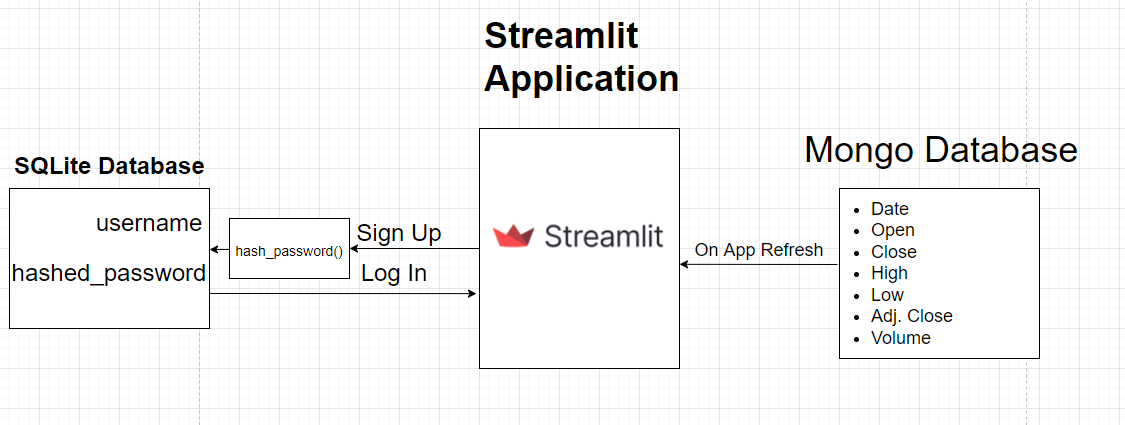
\includegraphics[scale=0.5]{img/architecture.png}
\end{center}

\subsection{Mongo Database}
\paragraph{The Mongo database stores the stock data of a collection of stocks. It stores date, open, close, high, low, adj. close, and volume. My Streamlit application then connects to the database with the following function.}

\begin{minted}{python}
def database(stock_selection):

    myclient = pymongo.MongoClient(connection_string)
    mydb = myclient["Stocks"]
    mycol = mydb[stock_selection]

    return mydb, mycol
\end{minted}

\paragraph{It takes whichever collection is currently selected by the user in a Streamlit select box. This reading of data is done each time the page is refreshed.}

\subsection{SQLite Database}
\paragraph{The SQLite database stores all data regarding the user. It holds the usernames and a hashed version of the password. User information is written to this SQLite database when the user creates an account. Data is then read from the database when the user attempts to log in. The hashed password is authenticated by taking in the password the attempted log in has given, hashing it using the same method as the initial hash and then comparing the two of these values.}

\begin{center}    
    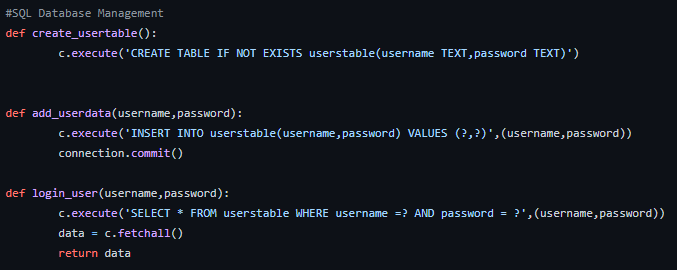
\includegraphics[scale=0.7]{img/sqlite.png}
\end{center}

\paragraph{The above is the functions used to initially create a user table, add user data to the database and login a user. As you can see the SQL queries are written in a fashion that resembles simple English. This makes it very clear for anyone reading the code to get a grasp of what the functions are doing very quickly. Below is the functions used to hash the password of the users and then check the hashed passwords when logging in. If the hashed password does match the hashed text from the input the log in is denied.}

\begin{center}    
    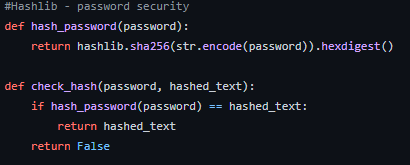
\includegraphics[scale=1]{img/hashlib.png}
\end{center}

\chapter{Conclusion}

\paragraph{This document has discussed my development of a web based application that allows for the creation of user accounts and user authentication. An application that takes in stock data from a Mongo database and displays this data in an aesthetically simple to understand manner via a well designed graph. This application also generates a forecasted prediction of the future success or failure of the stock chosen by the user by using a long short term memory based neural network. To build this application I had to use skills and knowledge I have obtained from my four years studying as a software development student. I also needed to learn a lot of new skills and acquire more knowledge during the development process.}

\subsection{Objectives}
\paragraph{As far as my objectives I am happy with the completion of these. Many of them took multiple tries using many different technologies to find the best fit. I completed all my initial objectives and done so to a standard I am happy with. To summarise, these were the objectives before I began my development.}

\begin{itemize}
    \item Develop a robust web application to a high standard using a technology that I have not yet developed with.
    \item Have my application read from and write to a database.
    \item Make my front-end user friendly and aesthetically pleasing for a good user experience.
    \item Allow users of the application to create accounts and log in to these accounts within the application
    \item Expand my knowledge of artificial intelligence, and more specifically machine learning techniques and applications.
    \item Develop an application in a manner similar to the industry standard like the agile methodology.
\end{itemize}

\paragraph{I am happy with my coverage of these objectives. Creating this application was certainly the most difficult venture of my college journey so far. Completing this project as the sole developer was difficult and time consuming. Meetings with my supervisor each week gave me a structure that was well needed to keep me on track with my development. I plan on expanding on my application in the future for personal enjoyment.}

\paragraph{My final remarks are that I enjoyed the work on this project and I am grateful to have had the opportunity to work on a project and write up to this scale and expand my knowledge on a variety of interesting topics.}